\bookchapter{Kapitel 42: Das Panorama der großen Modelle und die API in der Praxis}

\chapterintro{Die letzten Kapitel haben sich damit beschäftigt, wie du mit der KI zusammenarbeitest. Dieses Kapitel beantwortet eine noch grundlegendere Frage: „Welche KI? Und wie benutze ich sie?“ Das große Modell-Panorama vom August 2026 ist ungeheuer vielfältig – international liefern sich GPT, Claude und Gemini ein Dreikampf, in China blühen DeepSeek, Tongyi Qianwen, GLM, Kimi und Doubao nebeneinander auf. Jedes Modell hat seinen eigenen Charakter und seine Stärken: Die richtige Wahl halbiert deine Mühe, die falsche verdoppelt sie. Dieses Kapitel stellt dir diese Modelle nicht nur vor, sondern zeigt dir auch, wie du sie über eine API in deine eigenen Apps einbindest und wie du passend zu deinem Bedarf den richtigen Token-Plan (Nutzungspaket) wählst.}

\booksection{Die internationalen Leitmodelle: drei starke Anbieter}

Auf dem internationalen Markt der großen Modelle haben sich im August 2026 drei starke Anbieter etabliert: OpenAI (GPT-Serie), Anthropic (Claude-Serie) und Google (Gemini-Serie). Jeder hat einen deutlich eigenen Charakter – lass uns sie einen nach dem anderen kennenlernen.

\booksubsection{Die OpenAI-GPT-5.6-Serie: der rundum ausbalancierte Allrounder}

OpenAI hat die Welle der großen Modelle ausgelöst, und die GPT-Serie ist bis heute das weltweit am häufigsten genutzte Modell. Die im Juli 2026 erschienene GPT-5.6-Serie folgt einer Drei-Stufen-Strategie: das Flaggschiff GPT-5.6 Sol für anspruchsvolle Inferenz, das ausgewogene GPT-5.6 Terra für die Alltagsentwicklung und das leichte GPT-5.6 Luna für Szenarien mit hohem Aufkommen und niedrigen Kosten. Alle drei Modelle teilen sich ein Kontextfenster von 1,05 Mio. Token und unterstützen Bildeingabe, Funktionsaufrufe und strukturierte Ausgaben.

\begin{center}
\begin{tabularx}{\linewidth}{|X|X|X|X|X|}
\hline
\textbf{Modell} & \textbf{Positionierung} & \textbf{Eingabe (/Mio. Token)} & \textbf{Ausgabe (/Mio. Token)} & \textbf{Kontextfenster} \tabularnewline
\hline
GPT-5.6 Sol & Flaggschiff-Inferenz & 5,00 US\$ (ca. 36 RMB) & 30,00 US\$ (ca. 217 RMB) & 1,05 Mio. Token \tabularnewline
GPT-5.6 Terra & ausgewogen, Alltag & 2,50 US\$ (ca. 18 RMB) & 15,00 US\$ (ca. 109 RMB) & 1,05 Mio. Token \tabularnewline
GPT-5.6 Luna & leicht, niedrige Kosten & 1,00 US\$ (ca. 7 RMB) & 6,00 US\$ (ca. 44 RMB) & 1,05 Mio. Token \tabularnewline
\hline
\end{tabularx}
\end{center}

\begin{center}\small\color{gray}Preisliste der OpenAI-GPT-5.6-Serie (August 2026)\end{center}

Die Kernstärke der GPT-Serie ist die Ausgewogenheit – Inferenz, Programmieren, Schreiben, Multimodalität: keine auffällige Schwäche. Dazu kommen OpenAIs riesiges Plugin-Ökosystem und Entwickler-Community; Dokumentation und Werkzeugkette sind am vollständigsten. Für Situationen, in denen du nicht weißt, was du wählen sollst, ist GPT die Standardantwort, die „blind gewählt“ nie falsch liegt. Die Schwächen: Der Zugriff von China aus erfordert spezielle Netzwerkwege, das Chinesische klingt gelegentlich nach „Übersetzerton“, und die API-Preise liegen im mittleren bis hohen Bereich.

\textbf{Gute Nachricht}\par

OpenAI kündigte im August 2026 an, dass das Standardmodell für Gratisnutzer auf GPT-5.6 Luna angehoben wurde und unbegrenzte Text-Chats freigeschaltet sind. Das heißt: Die Grundfähigkeiten von GPT erlebst du ohne Kosten; zahlen musst du erst, wenn du stärkere Inferenz oder API-Aufrufe brauchst.

\booksubsection{Die Anthropic-Claude-Serie: die Spitze beim Programmieren und bei der Sorgfalt}

Wenn GPT der Allrounder ist, dann ist Claude beim Programmieren die „Messlatte“. Anthropics Claude-Serie führt beim SWE-bench (Software-Engineering-Benchmark) seit Langem mit klarem Abstand; Codequalität und die Fähigkeit, Projekte in Ingenieursqualität umzusetzen, sind Branchenspitze. Noch bemerkenswerter: Claude hat die niedrigste Halluzinationsrate (Wahrscheinlichkeit falscher Angaben) im gesamten Feld, nur etwa 1 \% – dadurch eignet es sich besonders für präzisionskritische Bereiche wie Wissenschaft und Recht.

Claudes zweiter Trumpf ist der extrem lange Kontext: ein Kontextfenster von 1 Mio. Token, mit dem sich mehrhundertseitige Verträge oder ganze Codebasen in einem Zug „durchlesen“ lassen, ohne Details zu verlieren. Beim Code-Refactoring, bei der Analyse langer Dokumente und Ähnlichem ist das praktisch unersetzlich. Claude Code, das Terminal-KI-Coding-Tool, erreichte bis Mitte 2026 einen annualisierten Umsatz von 2,5 Milliarden US-Dollar – der deutlichste Beleg dafür, wie anerkannt Claudes Programmierfähigkeit ist.

\begin{center}
\begin{tabularx}{\linewidth}{|X|X|X|X|X|}
\hline
\textbf{Modell} & \textbf{Positionierung} & \textbf{Eingabe (/Mio. Token)} & \textbf{Ausgabe (/Mio. Token)} & \textbf{Kontextfenster} \tabularnewline
\hline
Claude Fable 5 & Flaggschiff & 10,00 US\$ (ca. 72 RMB) & 50,00 US\$ (ca. 362 RMB) & 1 Mio. Token \tabularnewline
Claude Opus 4.8 & Profi-Modell & 5,00 US\$ (ca. 36 RMB) & 25,00 US\$ (ca. 181 RMB) & 1 Mio. Token \tabularnewline
Claude Sonnet 5 & Preis-Leistungs-Modell & 2,00 US\$ (ca. 14 RMB) & 10,00 US\$ (ca. 72 RMB) & 1 Mio. Token \tabularnewline
\hline
\end{tabularx}
\end{center}

\begin{center}\small\color{gray}Preisliste der Anthropic-Claude-Serie (August 2026; Sonnet 5 zum Aktionspreis)\end{center}

Claudes Schwäche ist der Preis – Fable 5 hat mit 50 US\$ pro Mio. Token den höchsten Ausgabepreis aller Modelle. Die Multimodal-Fähigkeiten (Bild- und Videoverständnis) sind ebenfalls relativ schwach. Für Einzelentwickler mit kleinem Budget ist Sonnet 5 in der Aktionsphase preislich äußerst attraktiv.

\booksubsection{Die Google-Gemini-Serie: der König der Multimodalität}

Googles Gemini-Serie ist 2026 bis zur Version 3.1 Pro weiterentwickelt. Geminis größter Trumpf ist die native Multimodalität – präzises Auswerten von Text und Bildern, fehlerfreie OCR-Tabellenerkennung, effizientes Extrahieren von Videoframes, dazu tiefgehende Analyse von Audio und Video. Es ist fest mit dem Google-Ökosystem (Suche, Mail, Cloud-Dienste) verzahnt und glänzt bei Echtzeit-Informationssuche und übergreifendem Modalitäten-Verständnis. Gemini unterstützt zudem eine Eingabe von bis zu 2 Mio. Token Kontext – aktuell das größte Kontextfenster überhaupt.

Gemini positioniert sich als „erste Wahl für wissenschaftliche Inferenz und Multimodal-Szenarien“. Wenn dein Projekt viel Bildanalyse, Videoverständnis oder wissenschaftliche Berechnung umfasst, hat Gemini kaum Gegner. Beim reinen Text-Codegenerieren liegt es allerdings leicht hinter Claude, und seine chinesischen Formulierungen wirken nicht so natürlich wie die der chinesischen Modelle.

\begin{center}
\begin{tabularx}{\linewidth}{|X|X|X|X|}
\hline
\textbf{Vergleichspunkt} & \textbf{GPT-5.6} & \textbf{Claude Fable 5} & \textbf{Gemini 3.1 Pro} \tabularnewline
\hline
Gesamtwertung & 94.8 & 95.0 & 92.1 \tabularnewline
Programmierfähigkeit (SWE-bench) & 74.9\% & 64.3\% (Pro) & Mittel \tabularnewline
Kontextfenster & 1,05 Mio. Token & 1 Mio. Token & 2 Mio. Token \tabularnewline
Multimodal-Fähigkeiten & ausgewogen & schwächer & am stärksten \tabularnewline
Halluzinationsrate & niedrig & am niedrigsten (ca. 1 \%) & niedrig \tabularnewline
Verfügbarkeit in China & Sonderzugang nötig & Sonderzugang nötig & Sonderzugang nötig \tabularnewline
API-Ökosystem & am ausgereiftesten & im Aufbau & an das Google-Ökosystem gebunden \tabularnewline
\hline
\end{tabularx}
\end{center}

\begin{center}\small\color{gray}Die drei großen internationalen Modelle im Vergleich (August 2026)\end{center}

\begin{tcbwarn}{Achtung: die praktische Hürde bei der Nutzung in China}
Für Entwickler in China ist die zentrale Hürde bei GPT, Claude und Gemini der Netzwerkzugang. Zwar lässt sich indirekt über Azure-Proxys oder API-Aggregationsplattformen arbeiten, doch Stabilität und Regelkonformität musst du selbst abwägen. Wenn dein Projekt strenge Anforderungen an die Datensicherheit stellt, lohnt es sich, zuerst heimische Modelle in Betracht zu ziehen.

\end{tcbwarn}

\booksection{Die chinesischen Leitmodelle: eine blühende Vielfalt}

Die großen chinesischen Modelle sind 2026 vom „Verfolger“ zum „Gleichauf-Läufer“ geworden und in manchen Feldern sogar zur „Spitze“. Anders als 2023, als ihnen der Vorwurf gemacht wurde, sie setzten nur auf fremde Modelle auf, stehen die chinesischen Flaggschiffe 2026 bei logischer Inferenz, Codeerzeugung und Chinesisch-Verständnis auf Augenhöhe mit den internationalen Top-Modellen – der Abstand ist auf unter 5 \% geschrumpft. Wichtiger noch: Bei chinesischen Szenarien, Kosten und regelkonformer Bereitstellung bieten sie unersetzbare Vorteile.

\booksubsection{DeepSeek V4: der König des Preis-Leistungs-Verhältnisses}

DeepSeek ist eine Erscheinung für sich unter den chinesischen Modellen. Anfang 2025 erschütterte DeepSeek-V3 den Markt mit dem Profil „ein Zehntel des GPT-Preises bei vergleichbarer Leistung“; die Branche nannte es die „K.-o.-Schwelle der Allzweck-KI“ – billiger als DeepSeek ist nichts so gut, teurer bietet nicht so viel fürs Geld. Im August 2026 erschien die finale Version DeepSeek V4-Pro: 1,6 Billionen Parameter im MoE-Aufbau, rund 49 Milliarden davon aktiv, 1 Mio. Token verlustfreier Kontext; beim Preis-Leistungs-Verhältnis für Code gilt es vielfach als weltweite Spitze.

DeepSeek V4 springt bei den Agent-Fähigkeiten deutlich nach vorn – der DeepSWE-Benchmark steigt von 12,8 auf 62,7 (+390 \%), NL2Repo von 38,5 auf 61,5. Die API unterstützt jetzt sowohl das Responses-API- als auch das Anthropic-API-Protokoll und ist damit kompatibel mit gängigen Coding-Tools wie Codex und Claude Code. Das heißt: Du kannst in Claude Code die DeepSeek-API statt der Claude-API nutzen – ein Bruchteil der Kosten bei fast identischem Erlebnis.

\begin{center}
\begin{tabularx}{\linewidth}{|X|X|X|X|X|}
\hline
\textbf{Modell} & \textbf{Positionierung} & \textbf{Eingabe (/Mio. Token)} & \textbf{Ausgabe (/Mio. Token)} & \textbf{Kontextfenster} \tabularnewline
\hline
DeepSeek V4 Pro & Flaggschiff-Inferenz & 3 RMB (ca. 0,43 US\$) & 6 RMB (ca. 0,87 US\$) & 1 Mio. Token \tabularnewline
DeepSeek V4 Flash & leicht und schnell & 1 RMB (ca. 0,14 US\$) & 2 RMB (ca. 0,28 US\$) & 1 Mio. Token \tabularnewline
\hline
\end{tabularx}
\end{center}

\begin{center}\small\color{gray}Preisliste der DeepSeek-V4-Serie (August 2026, Aktionspreise)\end{center}

Preisvergleich: Für je 1 Mio. Token Eingabe plus 1 Mio. Token Ausgabe zahlst du bei DeepSeek V4 Flash rund 0,42 US\$, bei GPT-5.6 Sol rund 35 US\$ und bei Claude Fable 5 rund 60 US\$ – ein Unterschied von bis zu 80- bis 140-fach.

\textbf{Stolperfalle: DeepSeek wird teurer}\par

DeepSeek hat am 6. August 2026 offiziell angekündigt, „in Kürze die API-Preise deutlich anheben zu wollen“ – die Aktionspreise dürften also nicht mehr lange gelten. In einzelnen Medien war vom bis zu 30-fachen die Rede; bis zum 14. August lag der endgültige Preisplan aber noch nicht vor. Außerdem führt die finale Version von DeepSeek V4 eine Spitzen-/Talzeit-Preisgestaltung ein – in Stoßzeiten verdoppeln sich die Aufrufpreise. Achte auf die offiziellen Ankündigungen für die aktuellsten Preise.

\booksubsection{Tongyi Qianwen Qwen3.7 Max: Alibaba Clouds Wahl für Unternehmen}

Die Tongyi-Qianwen-Serie (Qwen) von Alibaba Cloud profitiert vom Alibaba-Cloud-Ökosystem und hat bei Enterprise-Deployments klare Vorteile. Das im Juli 2026 erschienene Qwen3.7 Max ist das aktuelle Flaggschiff: ein dichtes Modell mit 235B Parametern, 256K nativem Kontext, erweiterbar auf 1M. Qwens Kernstärken: ein ausgereiftes Open-Source-Ökosystem (die ganze Serie von 7B bis 235B ist offen), präzises Verständnis chinesischer Szenarien und tiefe Integration in die Alibaba-Cloud-Infrastruktur.

\begin{center}
\begin{tabularx}{\linewidth}{|X|X|X|}
\hline
\textbf{Modell} & \textbf{Ausgabepreis (/Mio. Token)} & \textbf{Geeignet für} \tabularnewline
\hline
qwen-turbo & 0,6 RMB & schlichte Frage-Antwort, Textklassifikation, hohes Aufkommen \tabularnewline
qwen-long & 2,0 RMB & Verarbeitung extrem langer Kontexte (10M) \tabularnewline
qwen3.7-flash & 7,2 RMB & allgemeine Chats, Inhaltserstellung \tabularnewline
qwen3.7-plus & 12,0 RMB & Multimodalität (Bild + Video), chinesisches Schreiben \tabularnewline
qwen3.7-max & 36,0 RMB & Flaggschiff für Chinesisch, komplexe Aufgaben \tabularnewline
\hline
\end{tabularx}
\end{center}

\begin{center}\small\color{gray}Staffelpreise der Tongyi-Qianwen-Serie Qwen (August 2026)\end{center}

Qwen staffelt seine Preise – vom extrem günstigen qwen-turbo (Ausgabe 0,6 RMB/Mio. Token) bis zum Flaggschiff qwen3.7-max (Ausgabe 36 RMB/Mio. Token) deckt die Serie alles ab, vom leichten Frage-Antwort-Betrieb bis zu komplexer Inferenz. Für Unternehmen, die ohnehin Alibaba Cloud nutzen, ist Qwen die naheliegendste Integrationswahl.

\booksubsection{Zhipu GLM-5.1: chinesische Nummer 1 beim SWE-bench}

Die GLM-Serie von Zhipu AI glänzt 2026. GLM-5.1 holte beim SWE-bench den ersten Platz unter den chinesischen Modellen: eine MoE-Architektur mit 744B Parametern und 1 Mio. Token Kontext. Es versteht chinesische Semantik präzise und erlaubt in China regelkonforme, lokale Bereitstellung (On-Premise) – entscheidend für Finanz- und Behördenszenarien mit hohen Datensicherheitsanforderungen. GLM-5.1 kostet 6 RMB pro Mio. Token Eingabe und 24 RMB Ausgabe und liegt damit im Mittelfeld der chinesischen Modelle.

\booksubsection{Kimi K3: der König der extrem langen Texte}

Die Kimi-Serie von Moonshot AI ist für die Verarbeitung extrem langer Texte bekannt. Das im Juli 2026 erschienene Kimi K3 hat 2,8 Billionen Parameter und gehört bei vielen Bewertungen komplexer Aufgaben zur weltweiten Spitzenklasse. Kimis Kernszenarien: Analyse langer Codebasen und abrufgestützte Recherche in langen Dokumenten – es verarbeitet den Text eines ganzen Buchs oder den Code eines ganzen Projekts und glänzt bei „Nadel im Heuhaufen“-Suchaufgaben. Kimi ist relativ teuer (Ausgabe rund 12–20 RMB/Mio. Token), aber beim Preis-Leistungs-Verhältnis in Langtext-Szenarien kommt nichts an es heran.

\booksubsection{Doubao: ByteDances Allrounder}

ByteDances Doubao-Serie zeigte sich 2026 konstant stark. Doubao Seed 2.1 Pro ist das Flaggschiff von Volcengine mit 256K Kontext, im Praxistest konstant in der Gesamtleistung und mit hervorragendem Erlebnis in chinesischen Szenarien. Doubaos Vorteile: schon bei der Registrierung gibt es viele Gratis-Token, eine ausgereifte Integration ins Volcengine-Ökosystem und Preise in einer der niedrigsten Stufen des Landes. Für Einsteiger, die KI-Programmieren schnell ausprobieren wollen, ist Doubao die Einstiegswahl ohne Hürden.

\begin{center}
\begin{tabularx}{\linewidth}{|X|X|X|X|X|X|}
\hline
\textbf{Vergleichspunkt} & \textbf{DeepSeek V4} & \textbf{Qwen3.7 Max} & \textbf{GLM-5.1} & \textbf{Kimi K3} & \textbf{Doubao 2.1 Pro} \tabularnewline
\hline
Gesamtwertung & 87.5 & 89.7 & 90.5 & 88+ & 85+ \tabularnewline
Programmierfähigkeit & extrem stark & Stark & chinesische SWE-Nummer 1 & Stark & überdurchschnittlich \tabularnewline
Chinesisch-Verständnis & sehr gut & sehr gut & präzise & sehr gut & sehr gut \tabularnewline
Kontextfenster & 1 Mio. & 256K-1M & 1 Mio. & extrem lang & 256K \tabularnewline
Ausgabepreis (RMB/M) & 6 & 36 & 24 & 12-20 & 30 \tabularnewline
Open Source & MIT-Lizenz & ganze Serie offen & teilweise offen & geschlossen & geschlossen \tabularnewline
lokale Bereitstellung & ja & ja & ja & nein & nein \tabularnewline
\hline
\end{tabularx}
\end{center}

\begin{center}\small\color{gray}Die fünf großen chinesischen Modelle im Vergleich (August 2026)\end{center}

Ein wichtiger Trend: Das Gefühl einer „Generationenlücke“ zwischen chinesischen Modellen und GPT/Claude ist verschwunden. Bei logischer Inferenz und Mathematik-Wettbewerben liegen die chinesischen Flaggschiffe zu GPT-5 meist nur im einstelligen Punktabstand. Beim systematischen Architekturdenken und komplexer Ingenieurs-Inferenz bleibt Claude vorn – es liefert Architekturvorschläge mit mehr „Feingefühl“, während chinesische Modelle gelegentlich „lehrbuchhaft“ wirken. Bei chinesischen Szenarien, Kostenkontrolle und regelkonformer Bereitstellung haben sie aber klar die Oberhand.

\begin{center}
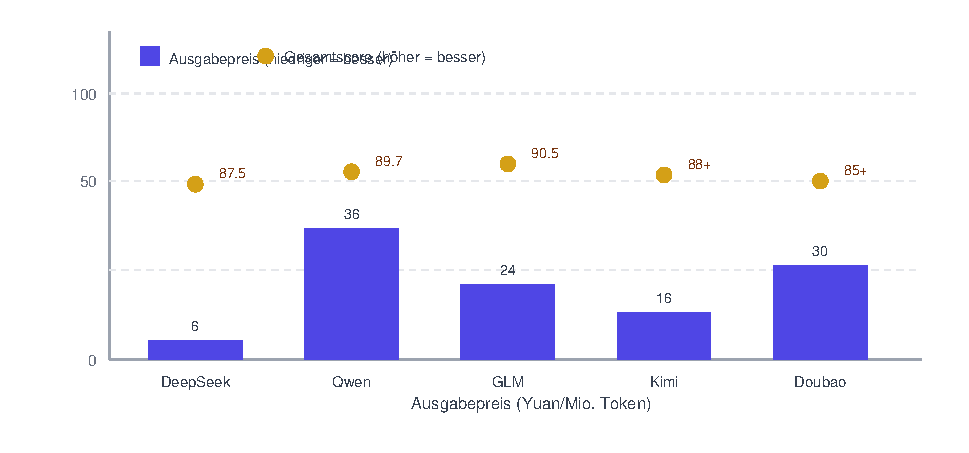
\includegraphics[width=0.92\linewidth]{figures/fig-di-si-shi-er-zhang-1}
\\[2pt]\small Abbildung 4: Preis- und Leistungsvergleich der fünf Modelle (niedrigerer Preis ist besser, höhere Punktzahl ist besser)
\end{center}

\booksection{Der Entscheidungsrahmen für die Modellwahl}

Nachdem du die Modelle kennst: Wie wählst du das richtige für dein Projekt? Hier bekommst du die „Vier-Fragen-Methode“ – beantwortest sie, hast du das passende Modell festgenagelt.

Läuft dein Projekt in China oder international?

In China heimische Modelle wählen

|

International ausländische Modelle möglich

Ist die Kernaufgabe Programmieren oder etwas anderes?

Programmieren Claude oder DeepSeek

|

Anderes weiter prüfen

Brauchst du sehr langen Kontext (>500 000 Token)?

Ja Gemini oder Kimi

|

Nicht nötig weiter prüfen

Budget knapp?

Knapp DeepSeek oder Qwen-turbo

|

Weniger kritisch GPT-5.6 oder Claude

\begin{center}\small\color{gray}Abbildung 5: Die Vier-Fragen-Entscheidungsmethode für die Modellwahl\end{center}

\begin{tcbinfo}{Tipp: Kombinationsstrategie}
Diese Methode ist kein Dogma – viele Szenarien brauchen eine Kombination mehrerer Modelle. Eine gängige Strategie: DeepSeek oder Qwen für die Alltagsentwicklung (günstig, gutes Chinesisch), Claude für kritische Architekturentscheidungen (starke Inferenz, wenig Halluzination), Gemini für Multimodal-Analysen (Bild- und Videobearbeitung). Wechsle das Modell nach Bedarf, statt stur bei einem Modell zu bleiben.

\end{tcbinfo}

\booksection{Erste Schritte mit der API: große Modelle von null anbinden}

Viele KI-Coding-Tutorials zeigen nur die Chat-Oberfläche. Aber echtes „KI-Programmieren“ – deine App ruft ein großes Modell auf – läuft über eine API. Eine API (Application Programming Interface, Programmierschnittstelle) ist ein Kommunikationsprotokoll zwischen Programmen. Über die API kann dein Code die Fähigkeiten eines großen Modells aufrufen, als riefe er eine Funktion auf.

\booksubsection{Was ist ein Token}

Bevor du die API verstehst, musst du den Begriff „Token“ begreifen. Token ist die Grundeinheit, nach der große Modelle abrechnen – denk an sie als „Lese- und Schreibeinheit der KI“. Ein Token entspricht etwa: im Englischen 0,75 Wörtern (4 Zeichen), im Chinesischen 0,5–1 Schriftzeichen. Ein chinesischer Text von 1000 Zeichen verbraucht etwa 1500–2000 Token.

Token sind weder Wortzahl noch Zeichenanzahl. Große Modelle zerlegen Text mit einem eigenen Tokenizer in Token. Dasselbe Wort kann je nach Modell unterschiedlich viele Token belegen – „Künstliche Intelligenz“ kostet in GPT vielleicht 3 Token, in DeepSeek vielleicht 2. Die APIs der meisten Modelle liefern die tatsächlich verbrauchte Tokenzahl zurück; du findest sie in der API-Antwort.

\begin{tcbinfo}{Token-Kosten schnell überschlagen}
1 Mio. chinesische Schriftzeichen entsprechen etwa 1,5 Mio. Token. Verarbeitest du 1 Mio. Zeichen Eingabe plus 1 Mio. Zeichen Ausgabe mit DeepSeek V4 Flash, kostet das rund 0,42 US\$ (ca. 3 RMB); mit Claude Fable 5 für dieselbe Menge rund 60 US\$ (ca. 434 RMB). Genau deshalb wirkt sich die Modellwahl direkt auf deine Projektkosten aus.

\end{tcbinfo}

\booksubsection{Den API-Key besorgen}

Der erste Schritt zur Nutzung der APIs großer Modelle ist der API-Key – eine Zeichenfolge zur Identitätsprüfung. Jeder Modellanbieter hat seine eigene API-Plattform; du registrierst ein Konto und legst einen API-Key an. Hier die Zugänge der API-Plattformen der wichtigsten Modelle samt Ablauf:

\begin{center}
\begin{tabularx}{\linewidth}{|X|X|X|X|}
\hline
\textbf{Modell} & \textbf{API-Plattform} & \textbf{Ablauf} & \textbf{Gratis-Kontingent} \tabularnewline
\hline
DeepSeek & platform.deepseek.com & Registrieren Identität verifizieren API-Key erstellen & Startguthaben für neue Nutzer \tabularnewline
Tongyi Qianwen & bailian.aliyun.com (Bailian-Plattform) & Mit Alibaba-Cloud-Konto anmelden Dienst aktivieren Key erstellen & Gratis-Testphase für neue Nutzer \tabularnewline
Zhipu GLM & open.bigmodel.cn & Registrieren Identität verifizieren API-Key erstellen & Startguthaben für neue Nutzer \tabularnewline
Kimi & platform.moonshot.cn & Registrieren Identität verifizieren API-Key erstellen & begrenztes Gratis-Kontingent \tabularnewline
Doubao & volcengine.com (Volcengine) & Registrieren Ark aktivieren API-Key erstellen & viele Gratis-Token bei der Registrierung \tabularnewline
OpenAI GPT & platform.openai.com & Registrieren Kreditkarte hinterlegen API-Key erstellen & kein Gratis-Kontingent (kostenpflichtig) \tabularnewline
Anthropic Claude & console.anthropic.com & Registrieren Karte hinterlegen API-Key erstellen & kleines Startguthaben für neue Nutzer \tabularnewline
\hline
\end{tabularx}
\end{center}

\begin{center}\small\color{gray}API-Plattformen der wichtigsten Modelle und Key-Bezug (August 2026)\end{center}

\textbf{Sicherheitshinweis: Der API-Key ist wie dein Wallet-Passwort}\par

Ein API-Key ist so wertvoll wie dein Wallet-Passwort – wer ihn hat, kann mit deinem Kontingent Modelle aufrufen. Deshalb: Schreibe den API-Key niemals in den Code (verwende Umgebungsvariablen); lade Code mit Key niemals in ein öffentliches Git-Repository; teile niemals Screenshots, auf denen der Key zu sehen ist. Wenn der Key abhandenkommt, lösch ihn sofort auf der Plattform und leg einen neuen an.

\booksubsection{Der erste API-Aufruf}

Mit deinem API-Key kannst du die API großer Modelle in jeder Programmiersprache aufrufen. Hier das einfachste Beispiel in Python – eine Nachricht an DeepSeek senden und die Antwort holen.

\begin{lstlisting}[language=Python]
# SDK installieren: pip install openai
# DeepSeek ist kompatibel mit dem OpenAI-SDK, direkt nutzbar
from openai import OpenAI
import os

# 1. Client erstellen (API-Key aus der Umgebungsvariable)
client = OpenAI(
    api_key=os.environ.get("DEEPSEEK_API_KEY"),
    base_url="https://api.deepseek.com"
)

# 2. Anfrage senden
response = client.chat.completions.create(
    model="deepseek-chat",  # Modell angeben
    messages=[
        {"role": "system", "content": "Du bist ein Python-Programmierassistent."},
        {"role": "user", "content": "Schreibe eine Quicksort-Funktion."}
    ]
)

# 3. Antwort abholen
print(response.choices[0].message.content)

# 4. Token-Verbrauch ansehen
print(f"Eingabe-Token: {response.usage.prompt_tokens}")
print(f"Ausgabe-Token: {response.usage.completion_tokens}")
print(f"Token gesamt: {response.usage.total_tokens}")
\end{lstlisting}

Die Kernlogik dieses Codes: Client anlegen (mit API-Key und Modelladresse) Nachrichtenliste bauen (system setzt die Rolle, user ist die Nutzereingabe) Anfrage senden Antwort holen. Dieses Muster passt auf praktisch alle Modelle im OpenAI-Format – um das Modell zu wechseln, tauschst du nur api\_key und base\_url. Genau deshalb orientieren sich viele chinesische Modelle am OpenAI-SDK-Format: Entwickler ändern zwei Zeilen Code, und das Modell wechselt – der Migrationsaufwand ist minimal.

Hier die Code-Unterschiede beim Wechsel auf andere Modelle – beachte, dass nur zwei Zeilen geändert werden:

\begin{lstlisting}[language=Python]
# DeepSeek
client = OpenAI(
    api_key=os.environ.get("DEEPSEEK_API_KEY"),
    base_url="https://api.deepseek.com"
)
# model="deepseek-chat"

# Qwen (Bailian-Plattform)
client = OpenAI(
    api_key=os.environ.get("DASHSCOPE_API_KEY"),
    base_url="https://dashscope.aliyuncs.com/compatible-mode/v1"
)
# model="qwen-plus"

# Zhipu GLM
client = OpenAI(
    api_key=os.environ.get("GLM_API_KEY"),
    base_url="https://open.bigmodel.cn/api/paas/v4"
)
# model="glm-4"

# OpenAI GPT
client = OpenAI(
    api_key=os.environ.get("OPENAI_API_KEY"),
    # Standard-base_url reicht
)
# model="gpt-5.6-terra"
\end{lstlisting}

\booksubsection{Streaming-Antworten verarbeiten}

In echten Anwendungen willst du meist nicht warten, bis die KI alles fertig geschrieben hat, um es auf einen Schlag zu zeigen – das lässt Nutzer zu lange warten. Gestreamte Antworten (Streaming) zeigen den Text Zeichen für Zeichen, während die KI ihn erzeugt, und heben das Nutzererlebnis deutlich. Wie bei einer Schreibmaschine, die Buchstabe für Buchstabe ausspuckt – für Nutzer fühlt sich das völlig anders an.

\begin{lstlisting}[language=Python]
# Streaming: Ausgabe Stück für Stück
stream = client.chat.completions.create(
    model="deepseek-chat",
    messages=[
        {"role": "user", "content": "Schreibe ein Tutorial zu Bubblesort in Python"}
    ],
    stream=True  # Streaming einschalten
)

# blockweise empfangen und ausgeben
for chunk in stream:
    if chunk.choices[0].delta.content is not None:
        print(chunk.choices[0].delta.content, end="", flush=True)
# die Ausgabe erscheint Buchstabe für Buchstabe wie bei einer Schreibmaschine
\end{lstlisting}

\booksection{Kaufberatung für Token-Pläne}

Die meisten Modellanbieter rechnen auf zwei Arten ab: nutzungsbasiert (Pay-as-you-go) und als Abo (Token-Plan/Subscription). Den Unterschied zu verstehen hilft dir, die Kosten deutlich zu senken.

\booksubsection{Pay-as-you-go vs. Abo}

\begin{center}
\begin{tabularx}{\linewidth}{|X|X|X|}
\hline
\textbf{Kriterium} & \textbf{Nutzungsbasiert (Pay-as-you-go)} & \textbf{Abo (Subscription)} \tabularnewline
\hline
Abrechnung & zahlen pro verbrauchtem Token & feste Vorauszahlung gegen Kontingent \tabularnewline
Geeignet für & schwankende Nutzung, gelegentliche Aufrufe & gleichmäßige Nutzung, häufige Aufrufe \tabularnewline
Preisvorteil & Standardpreis & 20–50 \% unter Nutzungsbasis \tabularnewline
Flexibilität & jederzeit nutzbar, ohne Bindung & Vorauszahlung nötig; Kontingent kann verfallen \tabularnewline
Überziehen & automatisch nutzungsbasiert & nach Aufbrauchen des Kontingents nutzungsbasiert \tabularnewline
Beispiel-Plattformen & die offiziellen API-Plattformen der Modelle & OpenAI Plus/Pro, Claude Pro, Cursor Pro \tabularnewline
\hline
\end{tabularx}
\end{center}

\begin{center}\small\color{gray}Vergleich der beiden Abrechnungsarten\end{center}

Für Einsteiger empfiehlt sich der Start mit nutzungsbasierter Abrechnung – keine Vorauszahlung, du zahlst nur, was du nutzt. Wenn sich deine Monatsnutzung auf einem Level einpendelt (etwa über 50 RMB pro Monat), denk über den Wechsel zum Abo nach, um den Stückpreis zu senken.

\booksubsection{Die wichtigsten Abo-Pakete im Überblick}

\begin{center}
\begin{tabularx}{\linewidth}{|X|X|X|X|}
\hline
\textbf{Paket} & \textbf{Monatspreis} & \textbf{Enthalten} & \textbf{Geeignet für} \tabularnewline
\hline
ChatGPT Free & gratis & unbegrenzte Text-Chats mit GPT-5.6 Luna & Erstkontakt ohne Vorkenntnisse \tabularnewline
ChatGPT Plus & 20 US\$/Monat & GPT-5.6 Sol, Bilderzeugung, Datenanalyse, Plugin-Zugang & Gelegenheitsnutzer \tabularnewline
ChatGPT Pro & 200 US\$/Monat & alle Modelle unbegrenzt, bevorzugter Zugang zu neuen Funktionen & Intensiv-Profis \tabularnewline
Claude Free & gratis & begrenzte Zahl von Claude-Chats & Erstkontakt ohne Vorkenntnisse \tabularnewline
Claude Pro & 20 US\$/Monat & Claude unbegrenzt, bevorzugter Zugang zu neuen Modellen & Entwickler \tabularnewline
Cursor Free & gratis & begrenzte KI-Vervollständigungen und Chats & für Anfänger zum Ausprobieren \tabularnewline
Cursor Pro & 20 US\$/Monat & unbegrenzte KI-Vervollständigungen, 500 Premium-Anfragen/Monat & Alltagsentwickler \tabularnewline
Cursor Business & 40 US\$/Monat pro Person & Teamzusammenarbeit, Admin-Bereich, Datenschutzmodus & für Teams \tabularnewline
\hline
\end{tabularx}
\end{center}

\begin{center}\small\color{gray}Abo-Pakete der wichtigsten KI-Tools (August 2026)\end{center}

Bei den chinesischen Modellen sehen die Abo-Angebote etwas anders aus. DeepSeek rechnet vor allem nutzungsbasiert ab und hat kein Monatsabo – du lädst Guthaben auf und zahlst nach tatsächlichem Verbrauch. Tongyi Qianwen bietet auf der Bailian-Plattform vorausbezahlte Ressourcenpakete (ein festes Token-Kontingent zum Rabattpreis). Doubao hat auf Volcengine ähnliche Vorauszahlungsangebote. Für Entwickler in China ist die sparsamste Kombination meist: DeepSeek nutzungsbasiert (Alltagsentwicklung) plus Doubaos Gratis-Kontingent (zum Ausprobieren).

\booksubsection{API-Aggregatoren}

Wenn du mehrere Modelle gleichzeitig nutzen willst, sind API-Aggregatoren eine bequeme Wahl. Eine Aggregatorplattform stellt dir einen einzigen API-Key bereit, mit dem du Dutzende Modelle aus aller Welt aufrufen kannst, ohne dich auf jeder Plattform separat zu registrieren.

\begin{center}
\begin{tabularx}{\linewidth}{|X|X|X|X|}
\hline
\textbf{Plattform} & \textbf{Merkmale} & \textbf{Preisvorteile} & \textbf{Geeignete Szenarien} \tabularnewline
\hline
OpenRouter (openrouter.ai) & Aggregator außerhalb Chinas: mit einem Key Modelle aus aller Welt aufrufen & Transparente Preise, Echtzeit-Preisvergleich möglich & Wenn du flexibel zwischen mehreren Übersee-Modellen wechseln willst \tabularnewline
SiliconFlow (siliconflow.cn) & Aggregator in China mit APIs für viele chinesische Modelle & 20–30 \% unter dem offiziellen Preis & Entwickler in China, die mehrere Modelle vergleichen wollen \tabularnewline
Azure OpenAI (Microsoft-Proxy) & Die über Microsoft Azure vermittelte OpenAI-API & Batch API mit 50 \% Rabatt & OpenAI auf Unternehmensniveau, große asynchrone Auftragsmengen \tabularnewline
Baidu Qianfan (qianfan.baidubce.com) & Baidus KI-Cloud-Plattform, mit Modellen wie Ernie (Wenxin) & Gratis-Guthaben für neue Nutzer & Nutzer im Baidu-Ökosystem \tabularnewline
\hline
\end{tabularx}
\end{center}

\begin{center}\small\color{gray}Die wichtigsten API-Aggregatoren (Stand: August 2026)\end{center}

\textbf{Vorsicht vor Fallen: Kaufe keine „Shared Keys“}\par

Kaufe keine sogenannten „Shared API Keys“ auf Plattformen wie Taobao oder Xianyu – diese Keys haben meist eine unklare Herkunft, können jederzeit gesperrt werden und bergen das Risiko von Datenlecks. Beziehe API-Keys immer über offizielle Plattformen oder seriöse Aggregatoren.

\booksubsection{Strategien zur Kostenoptimierung}

Das richtige Modell zu wählen ist nur der erste Schritt; sparsam damit umzugehen ist genauso wichtig. Hier einige praxiserprobte Strategien zur Kostenoptimierung:

\begin{enumerate}
  \item Nutze Cache-Treffer clever. Viele Modelle bieten eine „Cache“-Funktion – enthält deine Anfrage Inhalte, die schon zuvor verarbeitet wurden (z. B. den Systemprompt), wird dieser Teil nur zu einem extrem niedrigen Preis berechnet. Bei DeepSeek kostet ein Cache-Treffer nur 1/60 des normalen Preises. Feste Systemprompts an den Anfang der Nachrichtenliste zu stellen maximiert die Cache-Trefferquote.
  \item Gestaffeltes Routing – einfache Aufgaben mit günstigen Modellen erledigen, komplexe mit teuren. Zum Beispiel DeepSeek V4 Flash für die Textklassifikation (Ausgabe: 2 Yuan pro Million Token) und Claude für den Architekturentwurf (Ausgabe: 181 Yuan pro Million Token). In einem Projekt können 80 \% der Aufrufe mit dem günstigen Modell laufen.
  \item Begrenze die Ausgabelänge. Die API wird nach Ausgabe-Token abgerechnet – je länger die Ausgabe, desto teurer. In Szenarien, die keine langen Ausführungen brauchen, setze den Parameter max\_tokens, um die Ausgabe zu begrenzen und zu verhindern, dass die KI „zu viel um den heißen Brei redet“.
  \item Nutze die Batch API für Aufgaben ohne Echtzeitbedarf. Wenn du viele Aufgaben hast, die keine sofortige Antwort brauchen (etwa Massen-Annotation von Daten oder Dokumentzusammenfassungen), bekommst du mit der Batch API 50 \% Rabatt. OpenAI und Azure bieten diese Funktion beide an.
  \item Überwache den Token-Verbrauch. Die meisten API-Plattformen bieten ein Nutzungs-Dashboard. Schau regelmäßig nach, wie sich der Verbrauch verteilt, finde die Aufrufe mit dem höchsten Token-Verbrauch und optimiere gezielt dort. Eine kleine Anpassung am Prompt (etwa statt „Erkläre bitte ausführlich“ jetzt „Erkläre es bitte in 3 Sätzen“) kann 50 \% der Token sparen.
\end{enumerate}

\begin{center}
\begin{tabularx}{\linewidth}{|X|X|X|X|}
\hline
\textbf{Optimierungsstrategie} & \textbf{Ersparnis} & \textbf{Umsetzungsaufwand} & \textbf{Erläuterung} \tabularnewline
\hline
Cache-Treffer & bis zu 98 \% & Niedrig & Feste Inhalte an den Anfang der Nachrichten stellen \tabularnewline
Gestaffeltes Routing & 50\%-80\% & Mittel & Einfache Aufgaben mit dem günstigen Modell \tabularnewline
Ausgabelänge begrenzen & 30\%-60\% & Niedrig & Den Parameter max\_tokens setzen \tabularnewline
Batch API & 50\% & Niedrig & Batch-Verarbeitung für Aufgaben ohne Echtzeitbedarf \tabularnewline
Prompt-Optimierung & 20\%-50\% & Mittel & Prompts straffen, Redundanz reduzieren \tabularnewline
\hline
\end{tabularx}
\end{center}

\begin{center}\small\color{gray}Strategien zur Kostenoptimierung und ihre Wirkung (Stand: August 2026)\end{center}

\booksection{Praxis: Eine LLM-API in dein Projekt einbinden}

Beenden wir dieses Kapitel mit einer kompletten Praxisübung – einem „KI-Zusammenfassungs-Generator“: Der Nutzer gibt einen langen Text ein, und über eine LLM-API wird eine Zusammenfassung erzeugt. Diese Übung zeigt den kompletten Ablauf eines API-Aufrufs: Umgebungskonfiguration, API-Aufruf, Fehlerbehandlung, Kostenkontrolle.

\begin{lstlisting}[language=Python]
# ai_summarizer.py - KI-Zusammenfassungsgenerator
import os
from openai import OpenAI

# 1. Konfiguration (API-Key aus der Umgebungsvariable, nie hart kodiert)
client = OpenAI(
    api_key=os.environ.get("DEEPSEEK_API_KEY"),
    base_url="https://api.deepseek.com"
)

def summarize(text: str, max_length: int = 200) -> dict:
    """Erzeugt eine Textzusammenfassung

    Args:
        text: zu zusammenfassender Originaltext
        max_length: maximale Länge der Zusammenfassung (Token)

    Returns:
        dict: enthält Zusammenfassung und Token-Verbrauch
    """
    try:
        response = client.chat.completions.create(
            model="deepseek-chat",
            messages=[
                {
                    "role": "system",
                    "content": "Du bist ein Zusammenfassungsgenerator."
                               "Fasse den Text des Nutzers klar und knapp zusammen."
                               "Die Zusammenfassung hat höchstens 3 Sätze."
                },
                {
                    "role": "user",
                    "content": f"Fasse den folgenden Text zusammen:\n\n{text}"
                }
            ],
            max_tokens=max_length,  # begrenzt die Ausgabelänge
            temperature=0.3  # niedrige Temperatur = stabiler
        )

        return {
            "success": True,
            "summary": response.choices[0].message.content,
            "input_tokens": response.usage.prompt_tokens,
            "output_tokens": response.usage.completion_tokens,
            "total_tokens": response.usage.total_tokens
        }

    except Exception as e:
        return {
            "success": False,
            "error": str(e)
        }

# 2. Anwendungsbeispiel
if __name__ == "__main__":
    long_text = """
    (langen Text hier einfügen ...)
    """

    result = summarize(long_text)

    if result["success"]:
        print(f"Zusammenfassung: {result['summary']}")
        print(f"Verbrauchte Token: {result['total_tokens']}")
        # Kostenschätzung: DeepSeek V4 Flash
        cost = result['total_tokens'] * 0.000004  # $\approx$ 0,4 Cent je 1000 Token
        print(f"Geschätzte Kosten: {cost:.4f} Yuan")
    else:
        print(f"Fehler: {result['error']}")
\end{lstlisting}

Dieser Code verkörpert mehrere Best Practices für API-Aufrufe: Der API-Key wird über Umgebungsvariablen gelesen und niemals in den Code geschrieben; die Funktion hat klare Dokumentation und Typhinweise; mit max\_tokens ist die Ausgabelänge begrenzt; temperature steht auf einem niedrigen Wert (0,3) für stabilere Ausgaben; es gibt eine vollständige Fehlerbehandlung; und der Token-Verbrauch wird fürs Kosten-Tracking zurückgegeben. Wenn du die KI diesen Code schreiben lässt, kannst du ihr genau diese Anforderungen nennen – sie ist durchaus in der Lage, das umzusetzen.

Die Schlussbotschaft dieses Kapitels: Modelle sind die "Munition", die Methodik die "Taktik". Die richtige Munition erleichtert den Kampf, aber ohne gute Taktik gewinnt auch die beste Munition keinen Krieg. Du kennst jetzt die Stärken der Modelle und den API-Umgang – dein "Munitionsdepot" ist voll; wie du die Schlacht führst, entscheidet die Denkmethodik aus den vorigen Kapiteln.

\begin{tcbpractice}{Los geht's: Bringe deinen ersten API-Aufruf zum Laufen}
Registriere dich auf einer Plattform für chinesische Modelle (empfohlen: DeepSeek oder Zhipu, beide schenken Neukunden ein Startguthaben), erstelle einen API-Key, trage ihn in die System-Umgebungsvariablen ein (nicht in den Code!) und führe dann den obigen Code für den „ersten API-Aufruf“ aus. In dem Moment, in dem die Antwort der KI ausgegeben wird, hast du die Grenze zwischen „KI nutzen“ und „KI-Anwendungen bauen“ überschritten.

\end{tcbpractice}

\begin{tcbsummary}{Kapitelfazit}
\begin{itemize}
  \item Internationale Top 3: GPT-5.6 (der ausgewogene Allrounder), Claude (König des Programmierens + nur 1 \% Halluzinationsrate), Gemini (Multimodal-König + 2 Mio. Kontext)
  \item Chinesische Top 5: DeepSeek V4 (Preis-Leistungs-König, Preiserhöhungs-Ankündigungen beachten), Qwen3.7 (Unternehmensklasse), GLM-5.1 (Nr. 1 in China bei SWE), Kimi K3 (extrem lange Texte), Doubao (kostenloser Einstieg)
  \item Die Vier-Fragen-Methode: Wo läuft das Modell? Programmieren oder etwas anderes? Sehr langer Kontext? Budgetkritisch?
  \item Token sind die Abrechnungseinheit: 1 chinesisches Zeichen $\approx$ 1,5–2 Token; 1 Million Zeichen $\approx$ 1,5 Millionen Token
  \item API-Key = Wallet-Passwort: in Umgebungsvariablen verwalten, niemals hardcoden, nie zu Git hochladen
  \item Chinesische Modelle sind meist kompatibel zum OpenAI-SDK: Für einen Modellwechsel genügen zwei geänderte Zeilen, api\_key und base\_url
  \item Fünf Spartipps: Cache-Treffer nutzen, gestaffeltes Routing, Ausgabe begrenzen, Batch API, Verbrauch überwachen
\end{itemize}

\end{tcbsummary}
